% the abstract
\chapter*{Foreword}
\phantomsection
\addcontentsline{toc}{chapter}{Foreword}
\setlength\parindent{0pt}
\vspace{-1cm}
The big red button. It is every biologist's dream; a mythical and mystical red button that takes their raw data and transforms it magically into a \emph{Nature} paper ready for submission. Of course this is an unattainable dream, but there are many steps we can take to easy the burden of data analysis and decrease the
turnaround time between sample collection and manuscript submission.

The road towards the big red button is made up of many pieces, which when combined in the right way will server to demystify bioinformatics and reveal the final the final image; a world in which researchers are empowered to once again analyze their own data without needing specialist bioinformatics skills.


\begin{center}
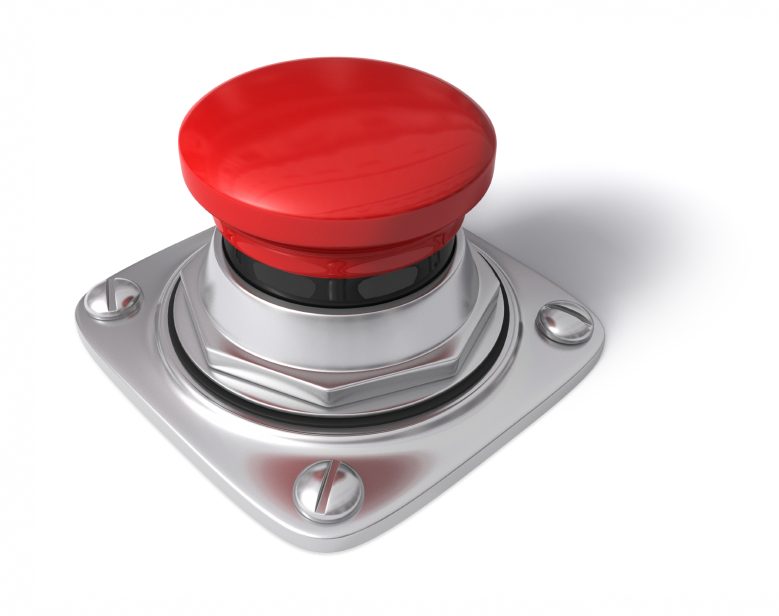
\includegraphics[scale=0.25]{chapters/images/redbutton.jpg}
\end{center}
